\documentclass[review]{elsarticle}

\usepackage{lineno,hyperref}
\modulolinenumbers[5]

\journal{Journal of \LaTeX\ Templates}

%%%%%%%%%%%%%%%%%%%%%%%
%% Elsevier bibliography styles
%%%%%%%%%%%%%%%%%%%%%%%
%% To change the style, put a % in front of the second line of the current style and
%% remove the % from the second line of the style you would like to use.
%%%%%%%%%%%%%%%%%%%%%%%

%% Numbered
%\bibliographystyle{model1-num-names}

%% Numbered without titles
%\bibliographystyle{model1a-num-names}

%% Harvard
%\bibliographystyle{model2-names.bst}\biboptions{authoryear}

%% Vancouver numbered
%\usepackage{numcompress}\bibliographystyle{model3-num-names}

%% Vancouver name/year
%\usepackage{numcompress}\bibliographystyle{model4-names}\biboptions{authoryear}

%% APA style
%\bibliographystyle{model5-names}\biboptions{authoryear}

%% AMA style
\usepackage{numcompress}\bibliographystyle{model6-num-names}

%% `Elsevier LaTeX' style
%\bibliographystyle{elsarticle-num}
%%%%%%%%%%%%%%%%%%%%%%%

\begin{document}

\begin{frontmatter}

\title{Autocategorization}

%% Group authors per affiliation:
\author{Andrew Carnes$^{1}$}
\address{$^1$University of Florida}

\begin{abstract}
In order to maximize the chance of discovering a certain effect, many scientific analyses extract subsets of data from the main data set that are sensitive to the effect. If the effect exists, the data in these sensitive subsets is expected to differ significantly from the null hypothesis. There are many ways to extract subsets, but an optimal method should minimize the global p-value on the null hypothesis given the effect. Call the orthogonal subsets of data categories and the selection of subsets categorization. An optimal categorization enhances the power of the experiment and reduces the data needed for discovery. By specifying a metric corresponding to the expected p-value (given the effect), the optimum categorization may be automated using a decision tree. This paper describes the autocategorization algorithm. 
\end{abstract}

%\begin{keyword}
%\texttt{elsarticle.cls}\sep \LaTeX\sep Elsevier \sep template
%\MSC[2010] 00-01\sep  99-00
%\end{keyword}

\end{frontmatter}

\linenumbers

\section{Introduction}

Many scientific analyses attempt to rule out a null hypothesis and declare a discovery. In this context, seeing a large enough discrepancy in the data from the null's prediction leads to a low p-value, the rejection of the null, and a discovery. With a model for the null and another for the expected data, the expected p-value can be quantified. An analysis with a lower p-value represents more convincing evidence to rule out the null, and therefore an analysis with a lower expected p-value is considered more sensitive. In addition, a more sensitive analysis requires less data to rule out the null hypothesis. For both of these reasons, optimizing the sensitivity is critical for any scientist.

The expected hypothesis and the null hypothesis determine probability density functions (PDFs) in a many dimensional feature space. However, data sparesly populates high dimensional spaces, and fits in high dimensions are difficult or untrustworthy in practice, so the PDFs are usually compared over a single discriminating feature - sometimes a few - to determine the p-value. Unfortunately, upon reducing to a lower dimensional PDF comparison, the sensitivity of the analysis is often reduced: feature space regions with large discriminating power are combined with those of high probability but low discrimination.

To regain sensitivity, the regions of feature space with large discriminating power need to be extracted. In this way, it makes sense to divide the feature space up into separate regions, called categories, and compare the low dimensional PDFs within the categories to maximize the sensitivity. By analytically specifying a metric corresponding to the expected p-value the optimum categorization can be automated. This is separate problem from regression or classification where fit values are applied to different regions of space to minimize some loss function. The goal is simply to divide up feature space to maximize the statistical sensitivity.

\section{The Autocategorizer Algorithm}
This section explains the autocategorization algorithm (autocategorizer) in terms of a binned counting experiment using histograms along a single variable, z. Let $H_o$ be the null hypothesis and $H_1$ be the expected hypothesis -- some trusted theory that probably generates the data. The goal of the autocategorizer is to partition feature space in order to minimize the expected p-value. Minimizing the expected p-value will maximize the chance for discovery if $H_1$ is indeed true.   

Let i label the bin and c label an orthogonal partition of feature space -- a category. Each category has its own histograms. Let $z_{c,i}$ describe the amount in the $i^{th}$ bin of the histogram for category c. Moreover, let $H_o$ predict $z_{c,i} = B_{c,i}$ in each bin for category c and let $H_1$ predict $z_{c,i} = S_{c,i} + B_{c,i}$ in each bin for category c.
\begin{figure}[hbp]
  \centering
  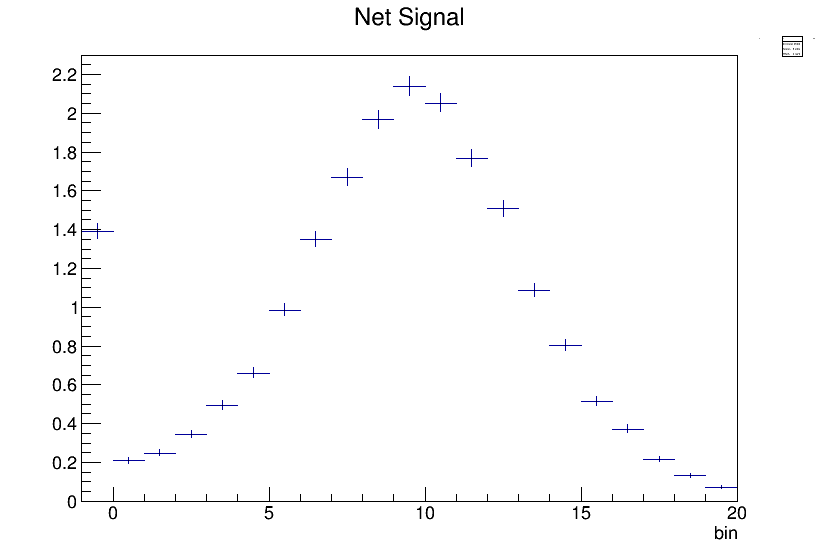
\includegraphics[width=0.49\linewidth]{binning_signal_example.png}
  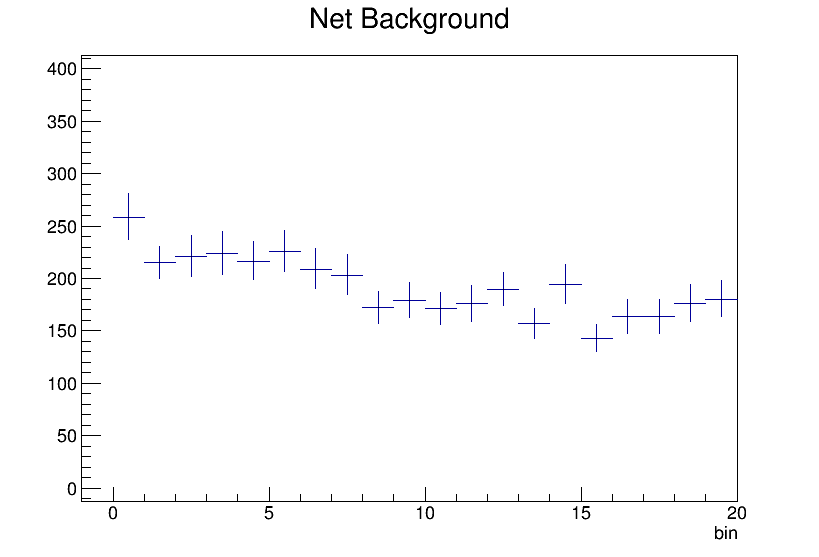
\includegraphics[width=0.49\linewidth]{binning_bg_example.png}
  \caption
  {An example of the S and B histograms in a category. The null hypothesis is given by B, and the expected hypothesis is given by S+B.}
  \label{fig:binning_example}
\end{figure}

The likelihood to observe $S_{c,i} + B_{c,i}$ in each bin when $B_{c,i}$ is expected in each bin provides a statistical measure of the discrepancy between $H_1$ and $H_o$. A low likelihood corresponds to a large discrepancy and a low p-value. Minimizing the likelihood will minimize the expected p-value. Equivalently, maximizing the negative log-likelihood (NLL) minimizes the expected p-value. The NLL for a single category's histogram is given by,  
\begin{equation}
\label{first}
-2log\left( p(z_{c,i}; \lambda_{c,i})/ C_{c,i} \right)  = -2log\left( \prod_{i} Poisson(z_{c,i}; \lambda_{c,i})/C_{c,i} \right),
\end{equation}
where the measured amount in a bin is given by $z_{c,i}$, and the amount expected by the hypothesis is given by $\lambda_{c,i}$. 

The categories are orthgonal, so the likelihoods for each category multiply, and the net NLL is  
\begin{equation}
\label{second}
-2log\left( p(z_i; \lambda_{c,i})/C_{c,i} \right) = -2log \left( \prod_{c,i} Poisson(z_{c,i}; \lambda_{c,i})/C_{c,i} \right) .
\end{equation}
Approximating each Poisson distribution by a Gaussian with $\mu_{c,i}=\lambda_{c,i}$ and $\sigma_{c,i}^2 = \lambda_{c,i}$, leads to a $\chi^2$ variable
\begin{equation}
-2log\left( \prod_{c,i} Poisson(z_{c,i}; \lambda_{c,i})/C_{c,i} \right) = \sum_{c,i}(z_{c,i}-\mu_{c,i})^{2}/\sigma^2_{c,i} 
= \sum_{c,i}(z_{c,i}-\lambda_{c,i})^{2}/\lambda_{c,i}.
\end{equation}
The factor of 2 in front of the log and the $C_{c,i}$ terms standardize the $\chi^2$ variable. To calculate the NLL to observe $H_1$ given $H_o$, $z_{c,i}$ is replaced by $S_{c,i} + B_{c,i}$, and $\lambda_{c,i}$ is replaced by $B_{c,i}$, 
\begin{equation}
{\rm Net~Significance} = \sum_{c,i}(z_{c,i}-\lambda_{c,i})^{2}/\lambda_{c,i} = \sum_{c,i}S_{c,i}^{2}/B_{c,i}.
\end{equation}
Choosing the categories to maximize the net significance will minimize the p-value. 

With the net significance acting as the metric, a decision tree\cite{cart84} can split up the feature space to maximize the metric. The decision tree algorithm greedily builds the optimum categorization by recursively splitting feature space regions into two using hyperplanes. 
\begin{figure}[hbp]
  \centering
  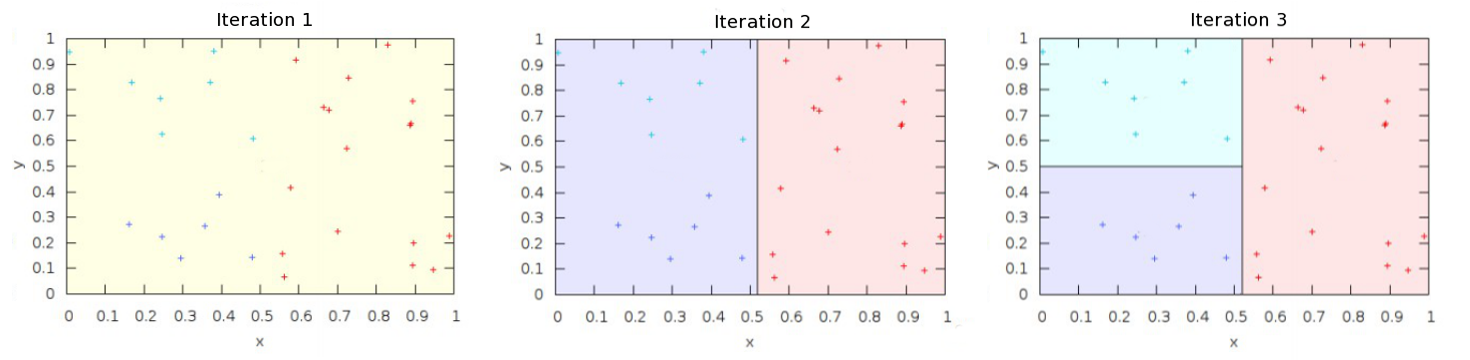
\includegraphics[width=0.98\linewidth]{iter_all.png}
  \caption
  {An example of the autocategorization process for features x,y and three categories. The autocategorizer chooses x=0.52 for the first split and y=0.50 for the second. The colored crosses represent the events that should be grouped together for optimum sensitivity. After three iterations, the categorizer correctly groups those events.}
  \label{fig:iter_example}
\end{figure}
On the first iteration, the autocategorizer calculates the net significance for the inclusive set of all events. The algorithm then searches over the inclusive set, checking all possible split values of the first feature, $x_1$. Events with $x_1$ values less than the split go in one candidate category, and those with $x_1$ values greater than or equal to the split value go into the other candidate category. 

For every split candidate, the algorithm calculates the net significance in the two categories delineated by the split value. The $x_1$ split value that provides the largest gain in significance over the inclusive set is stored along with the value of its gain. The gain is defined in Equation \ref{gain} where c1 and c2 are the prospective categories created from c by splitting on the feature.
\begin{equation}
{\rm Gain} = \sum_{i}S_{c1,i}^{2}/B_{c1,i} + \sum_{i}S_{c2,i}^{2}/B_{c1,i} - \sum_{i}S_{c,i}^{2}/B_{c,i} 
\label{gain}
\end{equation}
The autocategorizer then searches over the second feature, $x_2$, and stores the gain and split value of the best $x_2$ split. The process is repeated for all of the remaining features.

The algorithm chooses to split at the feature value with the largest gain, creating two
categories from the inclusive set of events. At the next iteration, the autocategorizer repeats the procedure for the two new
categories and chooses to split the category that provides the most gain. This process continues, each time greedily choosing to
split the category with the most gain, until the number of categories desired is reached.

The net sensitivity metric used above is just one approximation of the NLL. Other metrics that track the expected NLL/p-value may be used. For instance, adding the Asimov significance \cite{cowan}(Equation 97) of each bin in quadrature is another reasonable approach.

\section{Conclusions}
The autocategorizer algorithm automatically maximizes the chance to discover an effect of interest by extracting an optimal ensemble of sensitive regions from a multidimensional feature space. The algorithm has been used at the Compact Muon Solenoid (CMS) experiment at CERN to set limits on the Higgs particle's rate of decay to two muons \cite{cmshiggsmumu2017}. In the Higgs to dimuons analysis, the autocategorizer improves the upper limit on the rate of decay by 15\% compared to human expert categorization with the same simulated data and the same features. The improvement is equivalent to collecting 32\% more data.

\section*{References}

\bibliography{mybibfile}

\end{document}
